\documentclass{report}
\usepackage{homework}
\usepackage{url}
\solstrue

\usepackage{graphicx}
\graphicspath{{figures/}}

\renewcommand{\hmwkTitle}{Homework 7}

\begin{document}
\mktitle

\begin{problem}
Consider the following network of routers where the numbers above each link indicate link costs:
\begin{center}
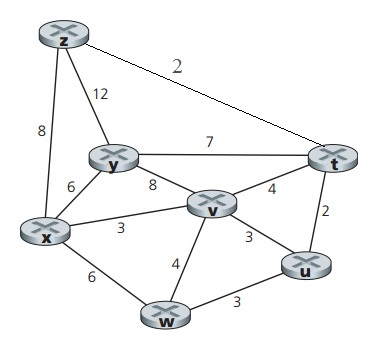
\includegraphics[scale = 0.7]{hw7-q1.jpg}
\end{center}

Considering calculations from the perspective of node \textbf{z}:

\begin{enumerate}
\item Show a table showing iterations of the Link State routing algorithm.
\item Show a resulting routing table (next hop for each destination).
\end{enumerate}


\begin{answer}{30em}
    \begin{enumerate}
    \item   \begin{tabular}[h]{|c|c|c|c|c|c|c|c|}
            \hline
            Step &
            N &
            y &
            x &
            v &
            t &
            w &
            u \\
            \hline
             & & & & & & & \\
             & & & & & & & \\
             & & & & & & & \\
             & & & & & & & \\
             & & & & & & & \\
             & & & & & & & \\
             & & & & & & & \\
             & & & & & & & \\
             & & & & & & & \\
             & & & & & & & \\
             & & & & & & & \\
             & & & & & & & \\
             & & & & & & & \\
             & & & & & & & \\
            \hline
            \end{tabular}
    \item \begin{tabular}{|c|c|}
    \hline
    Destination &   Next Hop \\ \hline
      &  \\
      &  \\
      &  \\
      &  \\
      &  \\
      &  \\\hline
    \end{tabular}
    \end{enumerate}
\end{answer}

\end{problem}



\newpage



\begin{problem}

Consider a network of 4 routers running Distance Vector routing algorithm where the numbers above each link indicate link costs.
\begin{center}
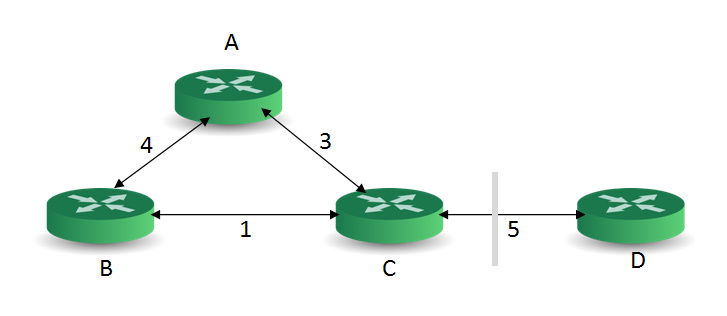
\includegraphics[scale=0.4]{hw7-q2.jpg}
\end{center}

\begin{enumerate}
\item Suppose, the link between C and D fails. Show that split horizon will not eliminate the count-to-infinity problem.
\item How can split horizon with poisoned reverse help in eliminating the count-to-infinity problem when the link between C and D fails?
\end{enumerate}

\begin{answer}{30em}
    Write your answer here
\end{answer}

\end{problem}


\newpage



\begin{problem}
Consider a simple network with one WiFi router and 3 hosts on the Figure.  Host A and B are connected to the router over wireless interface, host C is connected using wired Ethernet interface.


\begin{enumerate}
\item Assign IP (IPv4) addresses, network masks, and next hop gateways (where applicable) addresses so that all of them can communicate with each other.

Consider that have been given 131.179.196.32/27 address block and all assignments should be made from that block. \textbf{Your assignment must use the most conservative IP address allocation.} That is, assign IP addresses to hosts using as many network bits (the largest possible subnet mask) as possible.

\item Fill the content of the Host C's routing table, \textbf{without using the default route}.
\end{enumerate}

\vspace{1cm}

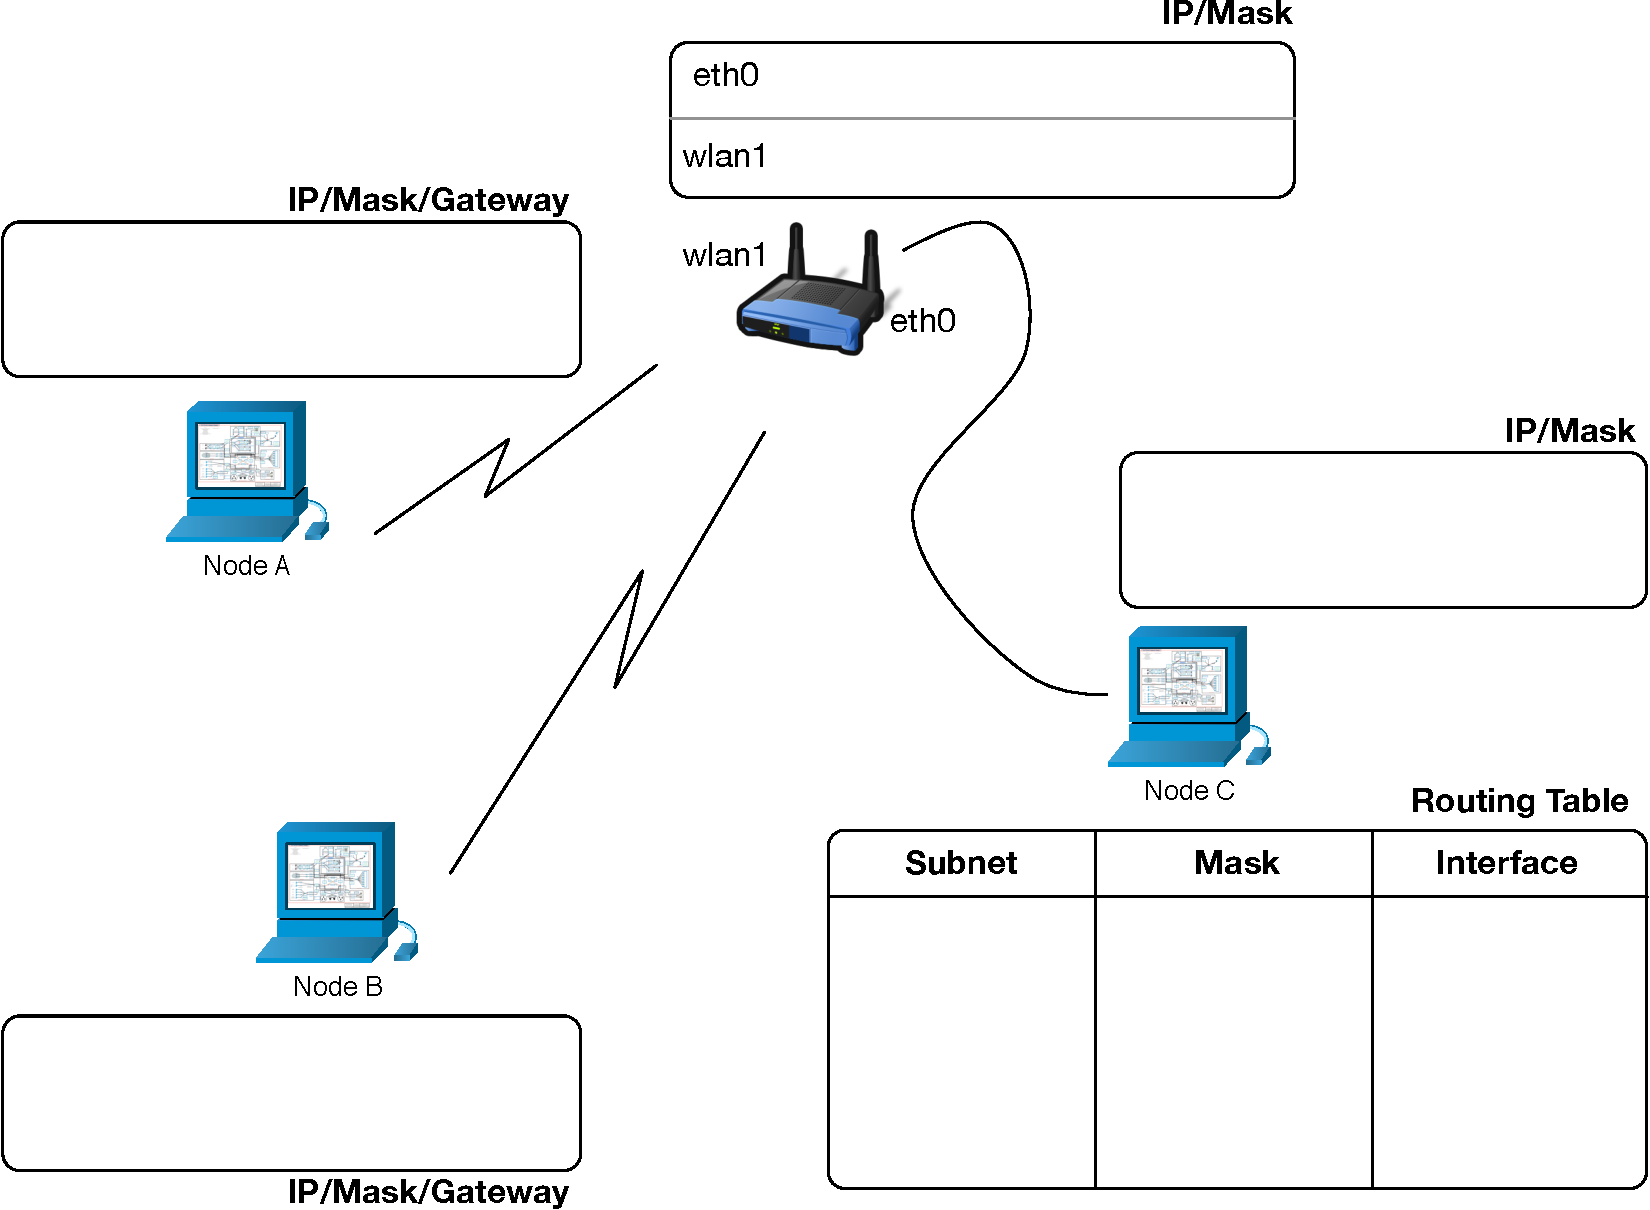
\includegraphics[scale=0.6]{hw7-topo.pdf}

\end{problem}



\newpage



\begin{problem}
Answer the following questions regrading to IP.
    
\begin{enumerate}
    \item Suppose Host A receives an IP datagram. How does the network layer in Host A know it should pass the segment (that is, the payload of the datagram) to TCP rather than to UDP or to something else?
    \item Can a host have more than one IP address? Justify your answer briefly.
    \item How does Skype work between two hosts which are behind two different NAT boxes?
    \item Compare IPv4 and IPv6 headers. What are the common fields?
\end{enumerate}


\begin{answer}{35em}
    Write your answer here
\end{answer}

\end{problem}

\newpage



\begin{problem}
Consider a network with four routers. Router A and D are IPv6 routers while router B and C are IPv4 routers. Assume that the source host sends an IPv6 packet to the destination host. The blue boxes in the figure represent the packet's location. Show source IP address and destination IP address of the packet located at (1) through (5).

\begin{center}
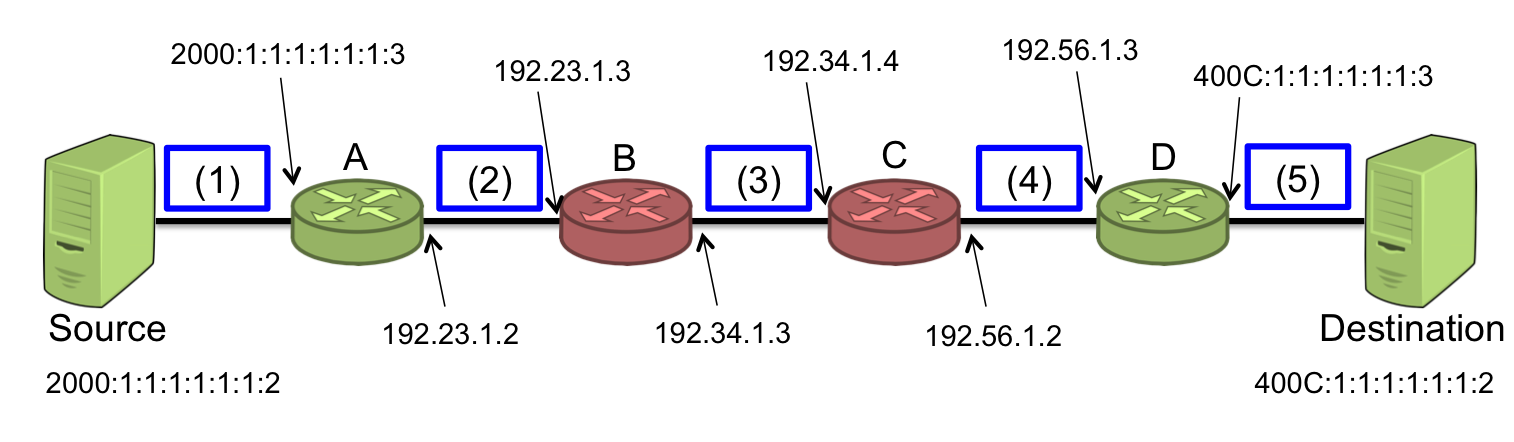
\includegraphics[width=\columnwidth]{hw7_p5.png}
\end{center}

\begin{answer}{35em}
    Write your answer here
\end{answer}

\end{problem}

\end{document}
